\documentclass[letterpaper]{article}

% --- Packages
\usepackage[utf8]{inputenc}
\usepackage[T1]{fontenc}
\usepackage[margin=0.25cm]{geometry}
\usepackage{enumitem}
\usepackage{pdfpages}
\usepackage{multicol}
\usepackage{amsmath}
\usepackage{amssymb}
\usepackage[skip=1pt plus1pt, indent=0pt]{parskip}
\usepackage{enumitem}
\usepackage{graphicx}

% --- Data
\title{Capacitance}
\author{Enrique Calderon}
\date{March 2024}

% --- Graphics path
\graphicspath{ {./img/} }

% --- Custom commands
\makeatletter
\let\thetitle\@title
\let\theauthor\@author
\makeatother
\newcommand{\compconj}[1]{%
    \overline{#1}%
}
\newcommand{\divline}{\noindent\makebox[\linewidth]{\rule{\textwidth}{0.4pt}}}
\newcommand{\taninv}{\tan^{-1}}
 
% Example of image adding
%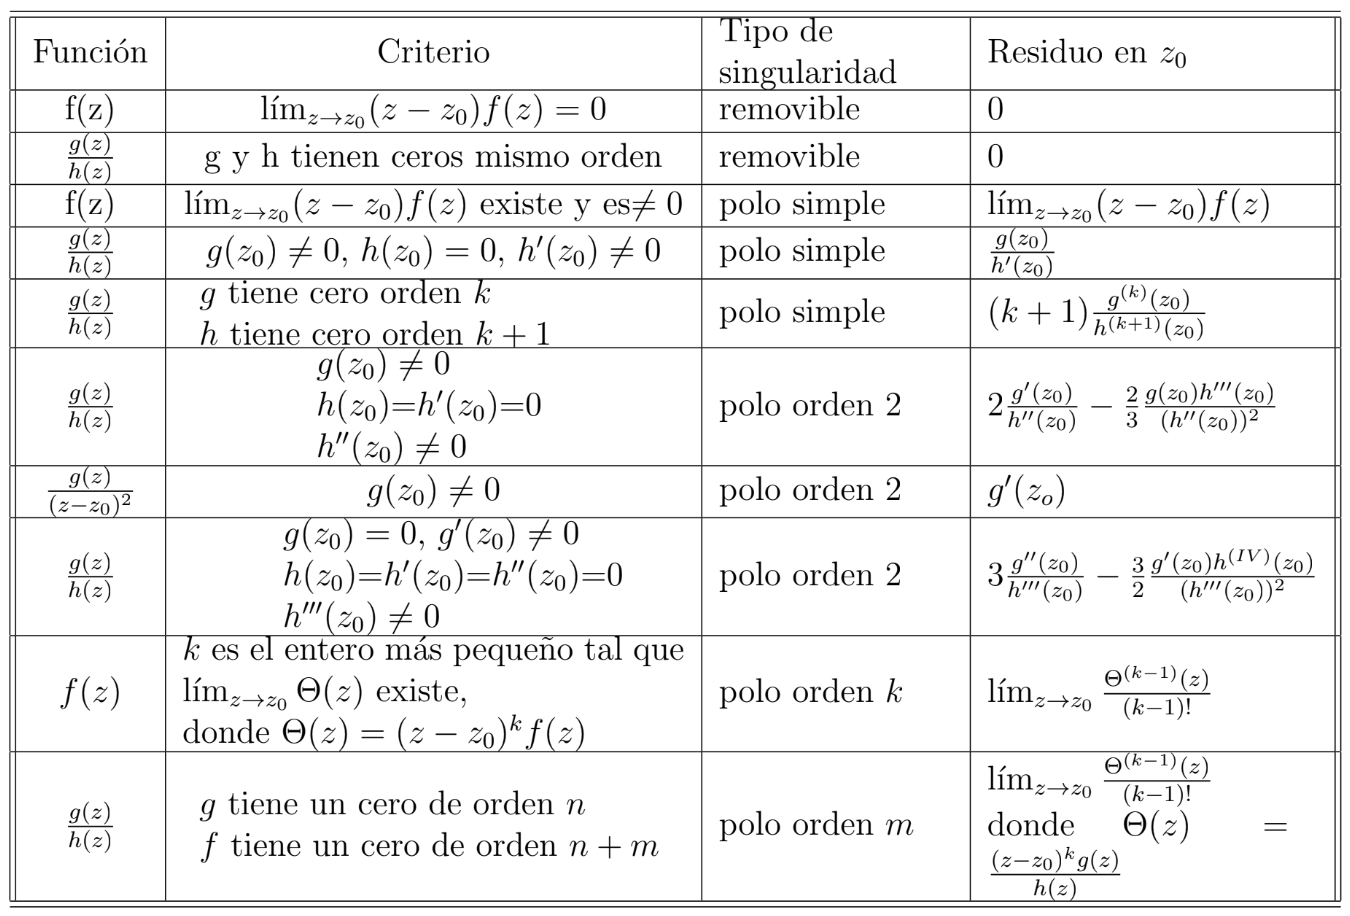
\includegraphics[width=0.8\textwidth]{ResidueTable}

% Remember to add divline between sections

\begin{document}
    \maketitle

    \divline
    \begin{multicols}{3}
        \section{Capacitance}

        By definitions:

        \[C = \frac{Q}{V_{\text{ab}}}\]

        With the units:

        \[ 1[F] = 1\frac{[C]}{[V]}\]

        Expanding:

        \[C = \epsilon_{0} \frac{A}{d} [F]\]
    \end{multicols}

    \divline
    \begin{multicols}{2}
        \section{Energy inside a capacitor}
        
        \[U_{c} = \frac{1}{2} \frac{Q^{2}}{C} [J]\]

        \[U_{c} = \frac{1}{2} C V^{2}_{\text{ab}} [J]\]
        
    \end{multicols}

    \divline
    \begin{multicols}{3}
        \section{Matter and electricity}

        Vector of dipole electrical moment:

        \[\overline{p}  = q_{i} \overline{l} [C \cdot m]\]

        Permittivity:

        \begin{align*}
            \epsilon_{\text{material}} &= k_{e} \epsilon_{0} &\left[ \frac{C^{2}}{N \cdot m^{2}} \right] \\
                &= \epsilon_{r} \epsilon_{0} &\left[ \frac{C^{2}}{N \cdot m^{2}} \right]
        \end{align*}

        Relative permittivity:

        \[k_{e} = 1 + x_{e} [1]\]

        Rupture electric field:

        \[E_{r} = \frac{V_{\text{max}}}{d} \left[ \frac{V}{m} \right]\]
    \end{multicols}

    \divline
    \begin{multicols}{2}
        \section{Electric vectors}

        Polarization vector:

        \begin{align*}
            \overline{P} &= \frac{Q_{i}}{A} \hat{u} &\left[ \frac{C}{m^{2}} \right] \\
                &= \sigma_{i} \hat{u} &\left[ \frac{C}{m^{2}} \right] \\
                &= \epsilon_{0} x_{e} \overline{E} &\left[ \frac{C}{m^{2}} \right] \\
                &= \epsilon_{0}(k_{e} - 1) \overline{E} &\left[ \frac{C}{m^{2}} \right]
        \end{align*}

        Displacement vector:

        \begin{align*}
            \overline{D} &= k_{e} \epsilon_{0} \overline{E} &\left[ \frac{C}{m^{2}} \right] \\
                &= \epsilon_{0} \overline{E} + \overline{P} &\left[ \frac{C}{m^{2}} \right]
        \end{align*}
    \end{multicols}

    \divline
    \begin{multicols}{2}
        \section{Capacitor connections}

        \subsection{Series}

        \[Q_{\text{ad}} = Q_{1} = Q_{2} = ...\]

        \[V_{\text{ab}} = V_{1} + V_{2} + ...\]

        \[C_{\text{eq}} = \left( \sum_{i = 1}^{n} \frac{1}{C_{i}} \right)^{-1} [F]\]

        \subsection{Parallel}

        \[Q_{\text{ad}} = Q_{1} + Q_{2} + ...\]

        \[V_{\text{ab}} = V_{1} = V_{2} = ...\]

        \[C_{\text{eq}} = \sum_{i = 1}^{n} C_{i} [F]\]
        
    \end{multicols}

    \divline
    \begin{multicols}{2}
        \section{Capacitor with dielectrics configuration}

        \subsection{Series}

        \[C_{1} = k_{1} \epsilon_{0} \frac{A_{1}}{d_{1}} [F]\]

        \[C_{2} = k_{2} \epsilon_{0} \frac{A_{2}}{d_{1}} [F]\]

        \[A = A_{1} = A_{2}\]

        \subsection{Parallel}

        \[C_{1} = k_{1} \epsilon_{0} \frac{A_{1}}{d_{1}} [F]\]

        \[C_{2} = k_{2} \epsilon_{0} \frac{A_{2}}{d_{1}} [F]\]

        \[\frac{1}{2} A = A_{1} = A_{2}\]
        
    \end{multicols}
\end{document}
